\begin{figure}
\centering
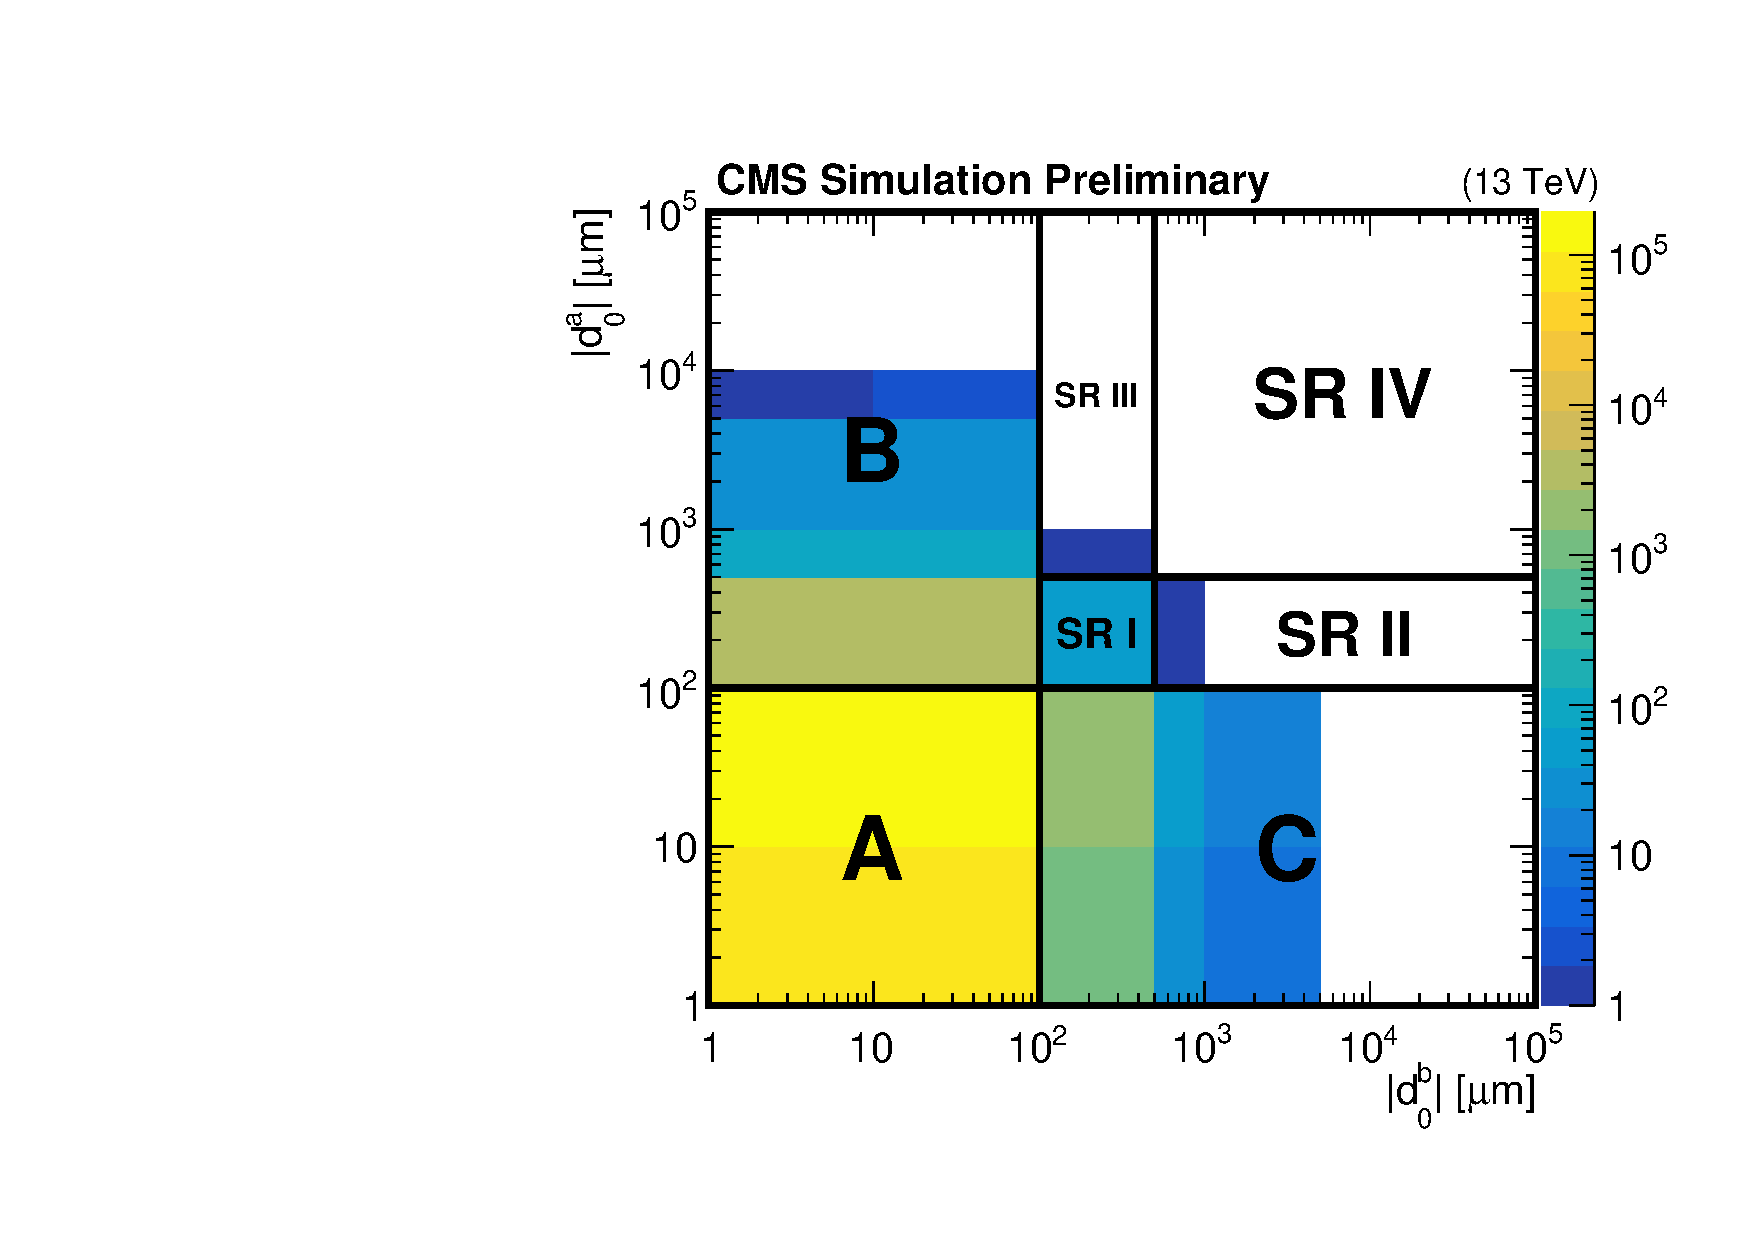
\includegraphics[width=0.8\textwidth]{figures/bg/abcdMethod_CMSPreliminary.pdf}
\caption{A diagram of the ABCD method overlaid on simulated background events passing the 2018 $\Pe\Pgm$ preselection. A, B, and C are control regions, and D corresponds to the inclusive SR, which includes SRs I, II, III, and IV. Underflow events are included in the bins along the left and bottom edges. When performing the background estimate, regions B and C are further subdivided to coincide with the SR for which the estimate is being performed.}
\label{abcd_regions}
\end{figure}